\subsection{Performance: Multiprocess Benchmarks} \label{sec:multiprocess-benchmarks}

\begin{figure}[thpb]
      \centering
      
    \begin{subfigure}[b]{\linewidth}
    \centering
    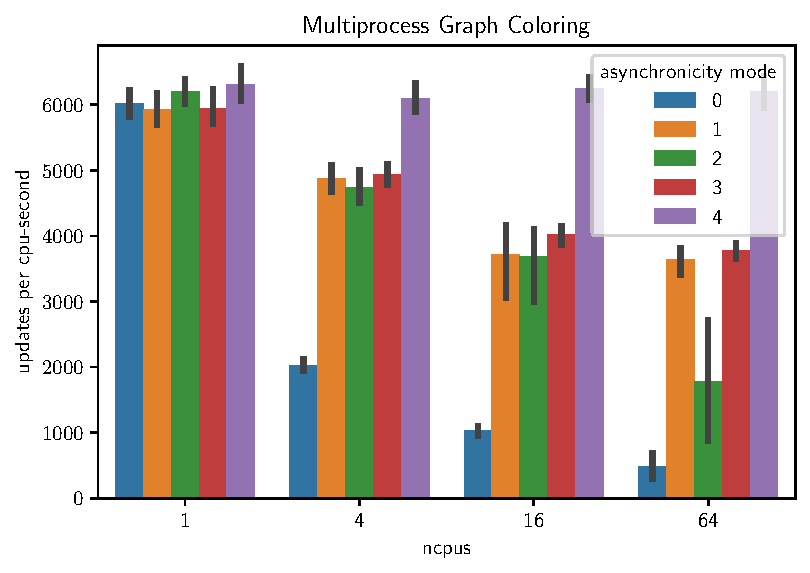
\includegraphics[width=\linewidth]{chart/multiprocess-graph-coloring}
    \caption{Graph coloring per-process update rate. Higher is better.}
    \label{fig:multiprocess_graph_coloring_update_rate}
    \end{subfigure}
    
    \begin{subfigure}[b]{\linewidth}
      \centering
      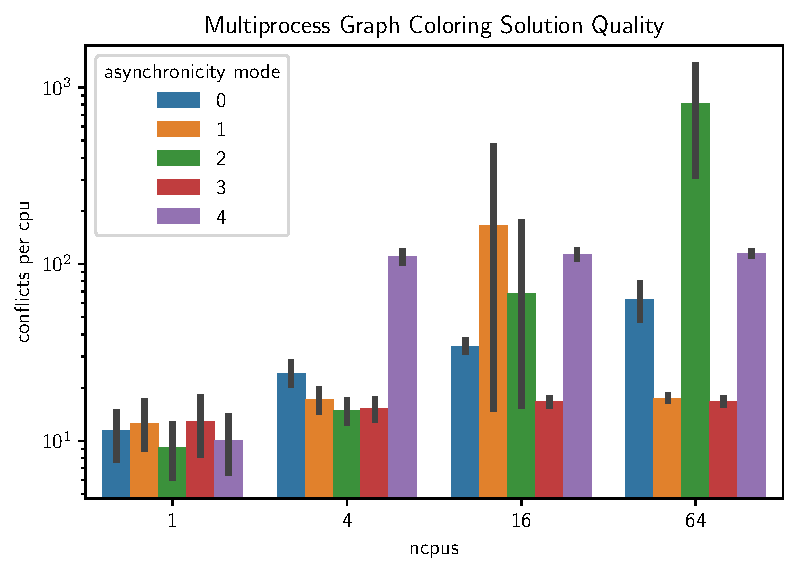
\includegraphics[width=\linewidth]{chart/multiprocess-graph-coloring-solution-quality} 
      \caption{Graph coloring solution conflicts. Lower is better.}
      \label{fig:multiprocess_graph_coloring_solution_quality}
    \end{subfigure}

  \begin{subfigure}[b]{\linewidth}
    \centering
  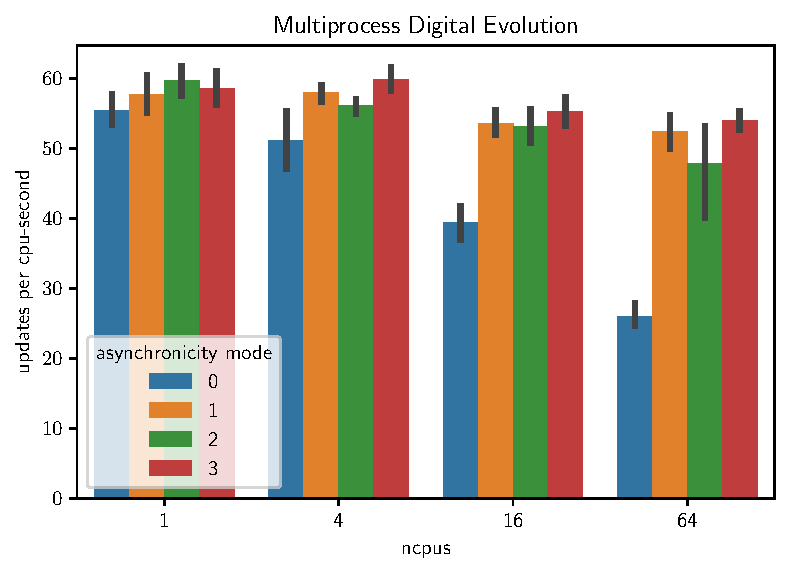
\includegraphics[width=\linewidth]{chart/multiprocess-digital-evolution}
  \caption{Digital evolution per-process update rate. Higher is better.}
  \label{fig:multiprocess_digital_evolution_update_rate}
  \end{subfigure}
      
  \caption{Multiprocess benchmark results. Bars represent bootstrapped 95\% confidence intervals. }
  \label{fig:multiprocess_benchmarks}
\end{figure}

Figure \ref{fig:multiprocess_graph_coloring_update_rate} shows per-cpu algorithm update rate for the graph coloring benchmark at 1, 4, 16, and 64 processes.
Unlike the multithreaded benchmark, multiprocess graph coloring exhibits consistent update-rate performance across process counts under asynchronicity mode 4, where inter-thread communication is disabled.
This matches the expectation that, indeed, with comparable hardware a single process should exhibit the same mean performance as any number of completely decoupled processes.
At 64 processes, best-effort asynchronicity mode 3 exhibits about 63\% the update-rate performance of single-process execution.
This represents about an $7.8\times$ speedup compared to fully-synchronous mode 0.
Indeed, best-effort mode 3 enables significantly better per-cpu update rates at 4, 16, and 64 processes ($p < 0.05$, non-overlapping 95\% confidence intervals).

Likewise, shown in Figure \ref{fig:multiprocess_graph_coloring_solution_quality}, best-effort asynchronicity mode 3 yields significantly better graph-coloring results within the allotted time at 4, 16, and 64 processes ($p < 0.05$, non-overlapping 95\% confidence intervals).
Interestingly, partial-synchronization modes 1 and 2 exhibited highly inconsistent solution quality performance at 16 and 64 process count benchmarks.
Fixed-timepoint barrier sync (mode 2) had particularly poor performance performance at 64 processes (note the log-scale axis).
We suspect this was caused by a race condition where workers would assign sync points to different fixed points different based on slightly different startup times (i.e., process 0 syncs at seconds 0, 1, 2... while process 1 syncs at seconds 1, 2, 3..).

Figure \ref{fig:multiprocess_digital_evolution_update_rate} presents per-cpu algorithm update rate for the digital evolution benchmark at 1, 4, 16, and 64 processes.
Relative performance fares well at high process counts under this relatively computation-heavy workload, with 64-process fully best-effort simulation exhibiting about 92\% the update rate of single-process simulation.
This represents a $2.1\times$ speedup compared to the fully-synchronous run mode 0.
Best-effort significantly mode 3 outperforms the per-cpu update rate of fully-synchronous mode 0 at process counts 16 and 64 ($p < 0.05$, non-overlapping 95\% confidence intervals).
